\documentclass[handout]{beamer}

% Lignes réponses
\usepackage{pgffor} % pour la commande \foreach permettant de réaliser une boucle
\newcommand{\pointilles}{{\\\rule{0pt}{1pt}\dotfill\rule{0pt}{1pt}}}
\newcommand{\rep}[1]{\foreach \n in {1,...,#1} {\pointilles}}

% Commandes pour cacher/révéler du texte facilement à l'aide d'un booléen
\usepackage{xstring}
\usepackage{ifthen}

\newboolean{reveal}
\setboolean{reveal}{false}

\newlength{\stextwidth} % une nouvelle longueur

\newcommand\x{6}

\newcommand{\guess}[1]{\ifthenelse{\boolean{reveal}}{{\color{red}#1}}{\settowidth{\stextwidth}{#1}\makebox[\stextwidth]{\dotfill}}}

\newcommand{\guessmath}[1]{\ifthenelse{\boolean{reveal}}{\textcolor{red}{#1}}{\settowidth{\stextwidth}{$#1$}\makebox[1.3\stextwidth]{\dotfill}}}

\newcommand{\guessmathbin}[1]{\ifthenelse{\boolean{reveal}}{\mathbin{\color{red}#1}}{\settowidth{\stextwidth}{$#1$}\makebox[2\stextwidth]{\dotfill}}}

% ========================================================================%

\usetheme{focus}

\usepackage{pgfpages}
\pgfpagesuselayout{4 on 1}[a4paper,landscape]

\usepackage[french]{babel}

\usepackage{xcolor}

\usepackage{pstricks,pst-plot,pst-text,pst-tree,pst-eps,pst-fill,pst-node,pst-math}
\usepackage{pstricks-add,pst-xkey}

\input ../tabvar

\usepackage{multicol}
\usepackage[np]{numprint}

\usepackage{booktabs}

\newcommand{\vect}[1]{\overrightarrow{#1}}
\newcommand{\Oij}{\left(O;\vect{i},\vect{j}\right)}
\newcommand{\norm}[1]{\left|\left|#1\right|\right|}

\begin{document}

\title{}

\date{}

\begin{frame}
  \frametitle{1. Représenter graphiquement une fonction}
  \textbf{Définition. --} Soit $f$ une fonction définie sur un ensemble $\mathcal{D}$. La courbe représentative $\mathcal{C}$ de $f$ dans un repère est l'ensemble des points de coordonnées $(x;y)$ telles que :

  \begin{center}
    $x$ appartient à \guess{$\mathcal{D}$} et $y=\guessmath{f(x)}$
  \end{center}

  \textit{Exemple. -- On a représenté ci-contre la fonction $f$ définie sur $[-4;3]$ par $f(x)=0,3x^3-4x+1$.}
\end{frame}

\begin{frame}
  \begin{center}
    \newrgbcolor{ccqqqq}{0.8 0. 0.}
    \psset{xunit=1.0cm,yunit=0.5cm,algebraic=true,dimen=middle,dotstyle=o,dotsize=5pt 0,linewidth=1.pt,arrowsize=3pt 2,arrowinset=0.25}
    \begin{pspicture*}(-5.,-6.)(4.,8.)
      \multips(0,-6)(0,2.0){8}{\psline[linestyle=dashed,linecap=1,dash=1.5pt 1.5pt,linewidth=0.4pt,linecolor=lightgray]{c-c}(-5.,0)(4.,0)}
      \multips(-5,0)(1.0,0){10}{\psline[linestyle=dashed,linecap=1,dash=1.5pt 1.5pt,linewidth=0.4pt,linecolor=lightgray]{c-c}(0,-6.)(0,8.)}
      \psaxes[labelFontSize=\scriptstyle,xAxis=true,yAxis=true,Dx=1.,Dy=2.,ticksize=-2pt 0]{->}(0,0)(-5.,-6.)(4.,8.)
      \psplot[linecolor=ccqqqq,plotpoints=200]{-4.0}{3.0}{0.3*x^(3.0)-4.0*x+1.0}
      \uput[ul](-4,-2.2){\color{ccqqqq}$\mathcal{C}$}
    \end{pspicture*}
  \end{center}
\end{frame}

\begin{frame}
  \textit{Exemple. -- Soit $g$ la fonction définie sur $[-2,5;2]$ par $g(x)=x^3-2x+1$. Grâce à la calculatrice, on obtient le tableau de valeurs ci-dessous :
    \begin{center}
      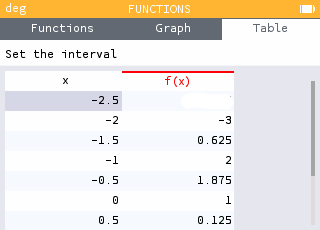
\includegraphics[width=5cm]{7_1_numworks.png}
    \end{center}
    \begin{enumerate}
      \item Quel nombre a été effacé ?\rep{1}
      \item Déterminer l'image de $1$, $1,5$ et $2$ par $g$.\rep{1}
      \item Représenter $g$ sur le graphique donné ci-contre.
    \end{enumerate}
  }
\end{frame}

\begin{frame}
  \psset{xunit=2.0cm,yunit=0.4cm,algebraic=true,dimen=middle,dotstyle=o,dotsize=5pt 0,linewidth=1.pt,arrowsize=3pt 2,arrowinset=0.25}
  \begin{pspicture*}(-3.,-12.)(2.5,6.)
    \multips(0,-12)(0,2.0){10}{\psline[linestyle=dashed,linecap=1,dash=1.5pt 1.5pt,linewidth=0.4pt,linecolor=lightgray]{c-c}(-3.,0)(2.5,0)}
    \multips(-3,0)(0.5,0){12}{\psline[linestyle=dashed,linecap=1,dash=1.5pt 1.5pt,linewidth=0.4pt,linecolor=lightgray]{c-c}(0,-12.)(0,6.)}
    \psaxes[labelFontSize=\scriptstyle,xAxis=true,yAxis=true,Dx=0.5,Dy=2.,ticksize=-2pt 0,subticks=2]{->}(0,0)(-3.,-12.)(2.5,6.)
    %\psplot[linewidth=1.pt,linecolor=blue,plotpoints=200]{-3.0}{2.5}{x^(3.0)-2.0*x+1.0}
  \end{pspicture*}
\end{frame}

\begin{frame}
  Pour tracer la courbe précédente, on a utilisé \guess{$10$} points. Afin d'obtenir une courbe plus \guess{\og{}précise\fg{}}, on pourrait utiliser davantage de points.
\end{frame}

\begin{frame}
  \frametitle{2. Savoir si un point appartient à la courbe d'une fonction}
  \textbf{Proposition. --} Avec les notations de la définition précédente :
  \begin{enumerate}
    \item Si $M(x;y)$ appartient à $\mathcal{C}_f$, alors $x$ appartient à $\mathcal{D}$ et $y=f(x)$.
    \item Si $x$ appartient à $\mathcal{D}$ et $y=f(x)$, alors $M(x;y)$ appartient à $\mathcal{C}_f$.
  \end{enumerate}

  \medskip

  \textit{Exemples. -- Soit $h$ la fonction définie sur $[-4;6]$ par $h(x)=2x^3-x+1$. On note $\mathcal{C}_g$ la courbe représentative de $h$ dans un repère du plan.
    \begin{enumerate}
      \item Le point $A(0;1)$ appartient-il à $\mathcal{C}_g$ ?\rep{2}
      \item Le point $B(2;16)$ appartient-il à $\mathcal{C}_g$ ?\rep{2}
    \end{enumerate}
  }
\end{frame}

\begin{frame}
  \frametitle{3. Reconnaître une fonction paire, une fonction impaire}
  \textbf{Définition. --} Lorsque dans un repère orthogonal, la courbe d'une fonction $f$ est symétrique par rapport à l'axe des ordonnées, on dit que la fonction $f$ est paire.

  \bigskip

  \textit{Exemple. -- On a représenté ci-contre la fonction carré, c'est-à-dire la fonction $k$ définie sur $\mathbb{R}$ par $k(x)=\guessmath{x^2}$. La fonction carré est \guess{paire}.}
\end{frame}

\begin{frame}
  \begin{center}
    \newrgbcolor{qqwuqq}{0. 0.39215686274509803 0.}
    \psset{xunit=1cm,yunit=1.0cm,algebraic=true,dimen=middle,dotstyle=o,dotsize=5pt 0,linewidth=1.pt,arrowsize=3pt 2,arrowinset=0.25}
    \begin{pspicture*}(-5.,-1.)(5.,7.)
      \multips(0,-1)(0,1.0){9}{\psline[linestyle=dashed,linecap=1,dash=1.5pt 1.5pt,linewidth=0.4pt,linecolor=lightgray]{c-c}(-5.,0)(5.,0)}
      \multips(-5,0)(1.0,0){11}{\psline[linestyle=dashed,linecap=1,dash=1.5pt 1.5pt,linewidth=0.4pt,linecolor=lightgray]{c-c}(0,-1.)(0,7.)}
      \psaxes[labelFontSize=\scriptstyle,xAxis=true,yAxis=true,Dx=1.,Dy=1.,ticksize=-2pt 0,subticks=2]{->}(0,0)(-5.,-1.)(5.,7.)
      \psplot[linewidth=1.pt,linecolor=qqwuqq,plotpoints=200]{-5.0}{5.0}{x^(2.0)}
    \end{pspicture*}
  \end{center}
\end{frame}

\begin{frame}
  \textbf{Définition. --} Lorsque dans un repère, la courbe d'une fonction $f$ est symétrique par rapport à l'origine du repère, on dit que la fonction $f$ est impaire.

  \bigskip

  \textit{Exemple. -- Soit $m$ la fonction cube, c'est-à-dire la fonction définie sur $\mathbb{R}$ par $m(x)=x^3$. Compléter le tableau de valeurs ci-dessous, puis représenter $m$ sur le graphique ci-contre :
    \begin{center}
      \begin{tabular}{@{}cccccccc@{}}
	\toprule
	$x$ & $-3$ & $-2$ & $-1$ & $0$ & $1$ & $2$ & $3$\\
	\midrule
	$m(x)$ &&&&&&&\\
	\bottomrule
      \end{tabular}
    \end{center}
  }

  \medskip

  \textit{On admettra que la courbe obtenue est symétrique par rapport à l'origine du repère. La fonction cube est donc une fonction \guess{impaire}.}
\end{frame}

\begin{frame}
  \begin{center}
    \newrgbcolor{ccqqqq}{0.8 0. 0.}
    \psset{xunit=1.0cm,yunit=0.1cm,algebraic=true,dimen=middle,dotstyle=o,dotsize=5pt 0,linewidth=1.pt,arrowsize=3pt 2,arrowinset=0.25}
    \begin{pspicture*}(-4.,-30.)(4.,30.)
      \multips(0,-30)(0,10.0){7}{\psline[linestyle=dashed,linecap=1,dash=1.5pt 1.5pt,linewidth=0.4pt,linecolor=lightgray]{c-c}(-4.,0)(4.,0)}
      \multips(-4,0)(1.0,0){9}{\psline[linestyle=dashed,linecap=1,dash=1.5pt 1.5pt,linewidth=0.4pt,linecolor=lightgray]{c-c}(0,-30.)(0,30.)}
      \psaxes[labelFontSize=\scriptstyle,xAxis=true,yAxis=true,Dx=1.,Dy=10.,ticksize=-2pt 0,subticks=2]{->}(0,0)(-4.,-30.)(4.,30.)
      %\psplot[linewidth=1.pt,linecolor=ccqqqq,plotpoints=200]{-4.0}{4.0}{x^(3.0)}
    \end{pspicture*}
  \end{center}
\end{frame}

\end{document}

%%% Local Variables:
%%% mode: latex
%%% TeX-master: t
%%% End:
